\documentclass[11pt]{article}

\usepackage{amsmath, amssymb}
\usepackage{geometry}
\usepackage{setspace}
\usepackage{enumitem}
\usepackage{graphicx}

\geometry{margin=1in}
\onehalfspacing

\title{\textbf{ECON 20100: Elements of Economic Analysis II}\\
Problem Set 1: Technology and Costs}
\date{Due: Wednesday, January 21, 2026}
\author{}

\begin{document}
\maketitle

\noindent \textbf{Instructions}
\begin{itemize}
    \item You may work in groups, but must submit individual solutions listing your group members.
    \item Show all work. Answers without justification will receive minimal credit.
    \item This problem set covers Sessions 1--4: Production functions, cost minimization, and cost curves.
\end{itemize}

\section*{Question 1: A Tale of Two Technologies (25 points)}

Two firms produce identical output but use different technologies:
\begin{align*}
\text{Firm A: } & f_A(K,L) = K^{1/4}L^{3/4} \\
\text{Firm B: } & f_B(K,L) = K^{2/3}L^{2/3}
\end{align*}

Input prices are $w = 12$ (wage) and $r = 4$ (rental rate of capital).

\begin{enumerate}[label=(\alph*)]
    \item \textbf{(4 points)} For each firm, determine the returns to scale. Show your work and provide economic intuition for what this implies about each firm’s cost structure.
    \item[] A: $f_A(tK,tL)=(tK)^{1/4}(tL)^{3/4}=t^{1/4+3/4}\cdot(K)^{1/4}(L)^{3/4}=t\cdot(K)^{1/4}(L)^{3/4}=t\cdot f_A(K,L)$
    \item[] B: $f_B(tK,tL)=(tK)^{2/3}(tL)^{2/3}=t^{2/3+2/3}\cdot(K)^{2/3}(L)^{2/3}=t^{4/3}\cdot(K)^{2/3}(L)^{2/3}=t^{4/3}\cdot f_A(K,L)$
    \item[] Both firms produce on a Cobb-Douglas production function where $f(\cdot)=K^\alpha L^\beta$. For firm A, $\alpha+\beta=1$ and thus firm A has constant returns to scale (CRS) meaning that cost rises proportionately to output. For firm B, $\alpha+\beta>1$ and thus firm B has increasing returns to scale (IRS) meaning that cost rises less proportionally to output (economies of scale).

    \item \textbf{(6 points)} Derive the cost-minimizing ratio $K/L$ for each firm. Which firm uses a more capital-intensive production process? Explain intuitively why this is the case, referencing the production function parameters.
    \item[] Cost minimization: $\min_{K,L}\; wL+rK$ st. $f(K,L)=\bar{y}$.
    \item[] A: $MP_L=\frac{3}{4}(K)^{1/4}(L)^{-1/4},\; MP_K=\frac{1}{4}(K)^{-3/4}(L)^{3/4}\Rightarrow\frac{MP_L}{MP_k}=3\cdot\frac{K}{L}=\frac{w}{r}\Rightarrow\frac{K}{L}=\frac{w}{3r}=1$
    \item[] B: $MP_L=\frac{2}{3}(K)^{2/3}(L)^{-1/3},\; MP_K=\frac{2}{3}(K)^{-1/3}(L)^{2/3}\Rightarrow\frac{MP_L}{MP_k}=1\cdot\frac{K}{L}=\frac{w}{r}\Rightarrow\frac{K}{L}=\frac{w}{r}=3$
    \item[] Firm B uses a more capital intensive production process. By the production function, a factor of $2/3$ is larger than a factor of $1/4$ on capital, and thus B is more capital intensive because capital contributes more to output. Similarly, when observing the cost-minimizing ratio $(\frac{K}{L})$, firm B uses more capital relative $(3>1)$ to labor for any given input prices $(w,r)$.

    \item \textbf{(8 points)} Suppose both firms must produce $y = 16$ units.
    \begin{enumerate}[label=(\roman*)]
        \item Find the cost-minimizing input bundle $(K^*, L^*)$ for each firm.
        \item[] A: $\frac{K}{L}=\frac{w}{3r}\Rightarrow K=\frac{w}{3r}L\Rightarrow16=(K)^{1/4}(L)^{3/4}=(\frac{w}{3r}L)^{1/4}(L)^{3/4}=(\frac{w}{3r})^{1/4}L\Rightarrow L=16(\frac{3r}{w})^{1/4}\Rightarrow K=\frac{w}{3r}L=\frac{16}{3}(\frac{w}{r})^{3/4}$
        \item[] Thus $(K^*,L^*)=(\frac{16}{3}(\frac{w}{r})^{3/4}, \; 16(\frac{3r}{w})^{1/4})=(\frac{16}{3}(3)^{3/4},\; 16)$
        \item[] B: $\frac{K}{L}=\frac{w}{r}\Rightarrow K=\frac{w}{r}L\Rightarrow16=(K)^{2/3}(L)^{2/3}=(\frac{w}{r}L)^{2/3}(L)^{2/3}=(\frac{w}{r})^{2/3}(L)^{4/3}\Rightarrow (L)^{4/3}=16(\frac{r}{w})^{2/3}\Rightarrow L=8(\frac{r}{w})^{1/2}\Rightarrow K=\frac{w}{r}L=8(\frac{w}{r})^{1/2}$
        \item[] Thus $(K^*,L^*)=(8(\frac{w}{r})^{1/2},\; 8(\frac{r}{w})^{1/2})=(8\sqrt{3},\; \frac{8}{\sqrt{3}})$
        \item Calculate the total cost for each firm.
        \item[] A: $C=wL+rK=12\cdot16+4\cdot\frac{16}{3}(3)^{3/4}=192+\frac{64}{3}(3)^{3/4}\approx240.6$
        \item[] B: $C=wL+rK=12\cdot\frac{8}{\sqrt{3}}+4\cdot8\sqrt{3}=\frac{96}{\sqrt{3}}+32\sqrt{3}\approx110.9$
        \item Which firm has lower costs? Is this surprising given your answer to part (a)? Explain.
        \item[] Firm B has the lower costs. Because firm B has increasing returns to scale it makes sense that cost is reduced at a higher levels of outputs compared to firm A. Further, firm B is more capital intensive as shown in part (b) and capital is cheaper $(4<12)$.
    \end{enumerate}

    \item \textbf{(7 points)} Now suppose the wage doubles to $w = 24$ while $r = 4$ remains unchanged. Without re-solving the entire problem, predict what happens to:
    \begin{enumerate}[label=(\roman*)]
        \item The $K/L$ ratio for each firm (increase, decrease, or stay the same?)
        \item[] $K/L$ increases for each firm by a factor of 2 because $K/L=(2w)/r\cdot\alpha/\beta$.
        \item Which firm is more affected by the wage increase in terms of percentage change in total cost? Justify your answer using economic reasoning about each firm’s factor intensity.
        \item[] Firm A is relatively labor-intensive while firm B is relatively capital-intensive. Thus, firm A is more strongly affected by the wage increase in terms of percentage change in total cost because it is more reliant on the wage input that is now more expensive.
    \end{enumerate}
\end{enumerate}

\section*{Question 2: The Geometry of Production (20 points)}

Consider the production function
\[
f(K,L) = \min\{2K, L\} + \sqrt{KL}.
\]

\begin{enumerate}[label=(\alph*)]
    \item \textbf{(5 points)} This production function combines elements of two ``standard'' production functions we studied. Identify them and explain what economic situation might give rise to such a technology. Provide an example of a company.
    \item[] This production function combines perfect compliments (Leontief) and Cobb-Douglas elements. Leontief arises when a firm has rigid input requirements in the production line. Cobb-Douglas arises when the firm has a more flexible process with input substitution. An example of a Leontief company might be a manufacturing plant where each machine requires 1/2 unit of labor. An example of Cobb-Douglas might be a brick-and-mortar customization shop where labor and capital are more interchangeable and case-dependent.

    \item \textbf{(6 points)} Consider the point $(K,L) = (4,8)$.
    \begin{enumerate}[label=(\roman*)]
        \item Calculate the output at this point.
        \item[] $f(4,8)=\min\{2(4),8\}+\sqrt{4(8)}=8+\sqrt{32}=8+4\sqrt{2}\approx13.7$
        \item Is this point on the ``kink'' of the Leontief component, or on one of the flat/vertical portions? What does this tell you about whether the firm has excess capital or labor from the Leontief component’s perspective?
        \item[] This point exists on the "kink" of the Leontief component because $2K=L$ exactly and the firm is balanced proportionately between capital and labor with no excess.
    \end{enumerate}

    \item \textbf{(9 points)} Suppose you’re at an interior point where $2K < L$ (so the Leontief part equals $2K$).
    \begin{enumerate}[label=(\roman*)]
        \item Write out the production function in this region.
        \item[] $f(K,L)=2K+\sqrt{KL}$ for $2K<L$
        \item Compute the marginal products $MP_K$ and $MP_L$ in this region.
        \item[] $MP_K=\frac{\partial f}{\partial K}=2+\frac{1}{2}(\frac{L}{K})^{1/2},\; MP_L=\frac{\partial f}{\partial L}=\frac{1}{2}(\frac{K}{L})^{1/2}$
        \item Does this production function exhibit diminishing marginal product of labor in this region? Prove your answer.
        \item[] $\frac{\partial MP_L}{\partial L}=\frac{1}{2}\cdot\frac{-1}{2}\cdot\frac{\sqrt{K}}{L^{3/2}}=-\frac{1}{4}\frac{\sqrt{K}}{L^{3/2}}<0$ for $K>0,\;L>0$ in this region
        \item[] Thus, the production function does exhibit diminishing marginal product of labor.
    \end{enumerate}
\end{enumerate}

\section*{Question 3: Short-Run Constraints (25 points)}

A bakery has the production function
\[
f(K,L) = 10K^{1/2}L^{1/2},
\]
where $K$ represents oven capacity (measured in rack-equivalents) and $L$ represents baker-hours. The wage is $w = 20$ per hour and the rental rate is $r = 5$ per rack-equivalent.

\begin{enumerate}[label=(\alph*)]
    \item \textbf{(5 points)} In the long run, find the cost-minimizing input ratio $K/L$ and the long-run cost function $C(y)$.
    \item[] $\min\; C=wL+rK=20L+5K$ st. $y=10K^{1/2}L^{1/2}\Rightarrow K^{1/2}L^{1/2}=\frac{y}{10}\Rightarrow KL=\frac{y^2}{100}$
    \item[] $MRTS_{KL}=\frac{MP_K}{MP_L}=\frac{\alpha}{\beta}\cdot\frac{L}{K}\Rightarrow\frac{1/2}{1/2}\cdot\frac{L}{K}=\frac{L}{K}=\frac{r}{w}=\frac{5}{20}=\frac{1}{4}$
    \item[] $\frac{L}{K}=\frac{1}{4}\Rightarrow K=4L\Rightarrow y=10(KL)^{1/2}=10(4L\cdot L)^{1/2}=10(4L^2)^{1/2}=10\cdot2L=20L$
    \item[] $\Rightarrow L^*=\frac{y}{20},\; K^*=4L=\frac{y}{5}\Rightarrow C(y)=wL^*+rK^*=20\cdot\frac{y}{20}+5\cdot\frac{y}{5}=y+y=2y$

    \item \textbf{(6 points)} Now suppose the bakery is stuck in the short run with $\bar{K} = 4$ oven racks.
    \begin{enumerate}[label=(\roman*)]
        \item Derive the short-run production function $y = g(L)$.
        \item[] $f_{SR}(\bar{K}=4,L)=10(\bar{K}L)^{1/2}=10(4L)^{1/2}=10(2)(L)^{1/2}=20\sqrt{L}$
        \item Derive the short-run total cost function $TC(y)$.
        \item[] $y=20\sqrt{L}\Rightarrow\sqrt{L}=\frac{y}{20}\Rightarrow L=\frac{y^2}{400}$
        \item[] $C_{SR}(y)=wL+r\bar{K}=20\cdot\frac{y^2}{400}+5\cdot 4=\frac{y^2}{20}+20$
        \item At what output level $y$ is the fixed capital $\bar{K} = 4$ actually optimal?
        \item[] From (a): $K^*=4L^*=\frac{y}{5}\Rightarrow\frac{y}{5}=4\Rightarrow y=20$, matches long-run optimal in short-run
    \end{enumerate}

    \item \textbf{(8 points)} Compute the following for the short-run cost function:
    \begin{enumerate}[label=(\roman*)]
        \item $MC(y)$
        \item[] $MC=\frac{dC}{dy}=\frac{d}{dy}(\frac{y^2}{20}+20)=\frac{y}{10}$
        \item $AVC(y)$
        \item[] $AVC=\frac{VC}{y}\Rightarrow VC=\frac{y^2}{20}\Rightarrow AVC=\frac{y^2/20}{y}=\frac{y}{20}$
        \item $ATC(y)$
        \item[] $ATC=\frac{C}{y}=\frac{(y^2/20)+20}{y}=\frac{y}{20}+\frac{20}{y}$
        \item Find the output level that minimizes $ATC$. Verify that $MC = ATC$ at this point.
        \item[] $\frac{dATC}{dy}=\frac{d}{dy}(\frac{y}{20}+\frac{20}{y})=\frac{1}{20}-\frac{20}{y^2}=0\Rightarrow\frac{1}{20}=\frac{20}{y^2}\Rightarrow y^2=400\Rightarrow y^*=20$
        \item[] $ATC(20)=\frac{y}{20}+\frac{20}{y}=\frac{20}{20}+\frac{20}{20}=1+1=2\iff MC(20)=\frac{y}{10}=\frac{20}{10}=2$
    \end{enumerate}

    \item \textbf{(6 points)} Sketch a graph showing $MC$, $AVC$, $ATC$, and $AFC$. Label:
    \begin{enumerate}[label=(\roman*)]
        \item The output level where $ATC$ is minimized
        \item The output level where the short-run capital is ``just right''
        \item[]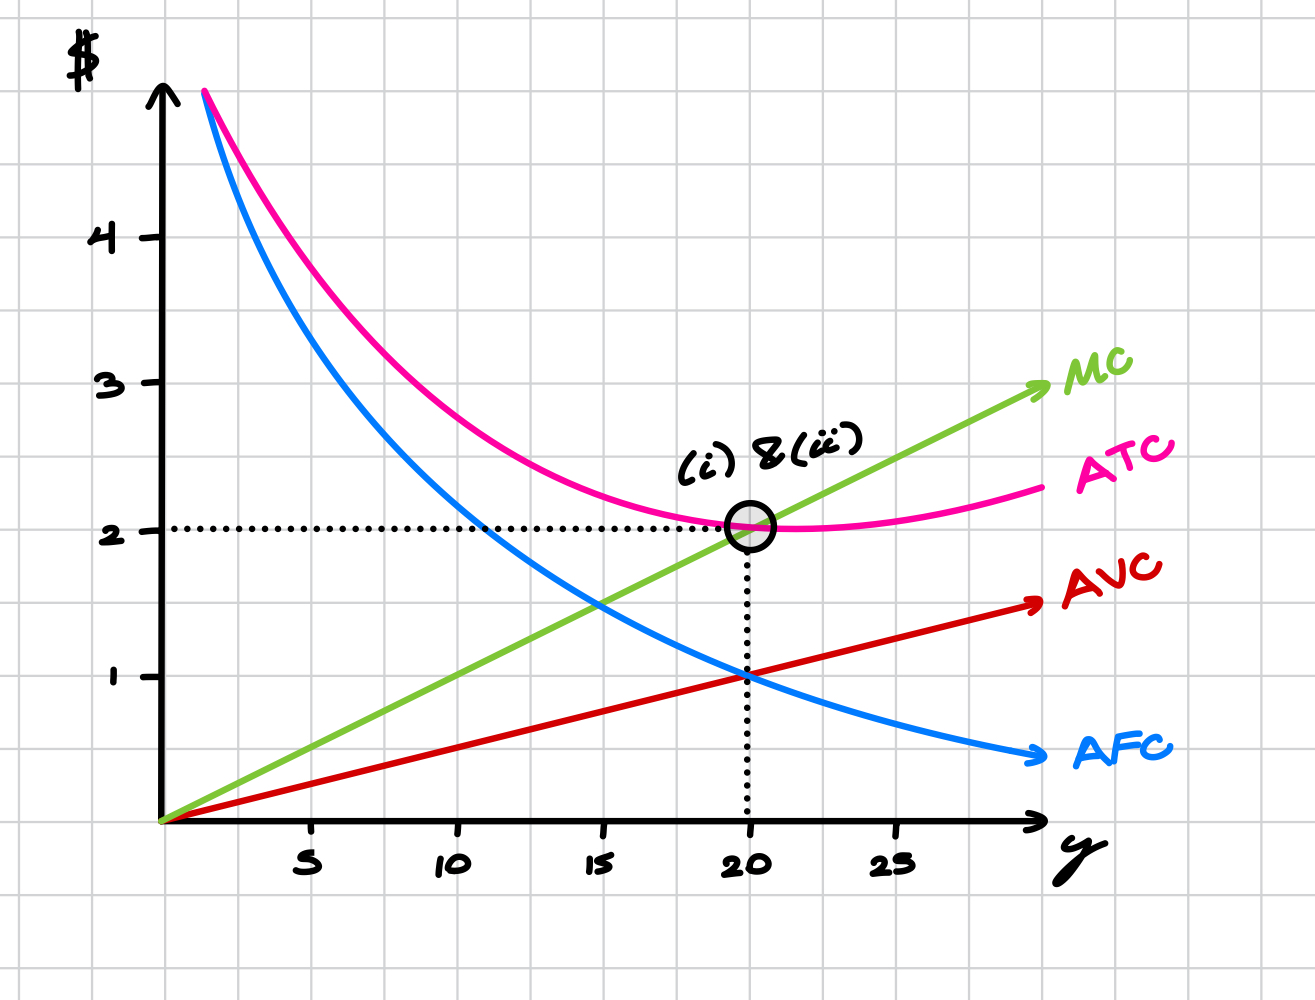
\includegraphics[width=10cm]{ECON 20100 PSet 1 Image 1.jpeg}

        \item Are these the same point? Explain why or why not.
        \item[] Yes, in this case these are the same point. $MC$ crosses $ATC$ at its minima because at an efficient scale production happens at the lowest possible cost per unit given short-run fixed capital ("just right" corresponding to long-run cost minimizing the $K/L$ ratio).
    \end{enumerate}
\end{enumerate}

\section*{Question 4: The Envelope in Action (15 points)}

A firm’s long-run average cost is given by
\[
LAC(y) = 100 - 10y + y^2 \quad \text{for } y \ge 0.
\]

\begin{enumerate}[label=(\alph*)]
    \item \textbf{(3 points)} Find the minimum efficient scale (MES). What is the minimum value of $LAC$?
    \item[] $\frac{dLAC}{dy}=-10+2y=0\Rightarrow2y=10\Rightarrow y=5=MES$
    \item[] $LAC(5)=100-10(5)+(5)^2=100-50+25=75=\text{minimum} \; LAC$

    \item \textbf{(4 points)} For output levels below the MES, does this firm exhibit economies or diseconomies of scale? What about above the MES?
    \item[] When $y<5$ below the $MES$, $\frac{dLAC}{dy}=-10+2y<-10+10=0$. Thus, $LAC$ is decreasing and the firm has economies of scale. When $y>5$ above the $MES$, $\frac{dLAC}{dy}=-10+2y>-10+10=0$. Thus, $LAC$ is increasing and the firm has diseconomies of scale.

    \item \textbf{(8 points)} Now consider the short run. Capital is fixed at the level optimal for $y^* = 5$.
    \begin{enumerate}[label=(\roman*)]
        \item What is this firm’s $ATC$ at $y = 5$?
        \item[] At $y=5$, $y=MES$, the firm is using the optimal amount of capital to produce efficiently. Thus, $ATC=LAC$ at $y=5$ so $ATC_{SR}(y=5)=75$.
        \item If demand increases and the firm produces $y = 7$, will $ATC(7)$ be higher or lower than $LAC(7)$? Explain.
        \item[] $ATC_{SR}(y=7)> LAC(7)$ because $LAC$ is the minimum $ATC$ if all inputs are adjustable. Here, since capital is fixed optimally for $y=5$ but $y>y^*$, the firm cannot adjust capital to minimize costs in the short run to account for additional output.
        \item If demand drops and the firm produces $y = 3$, will $ATC(3)$ be higher or lower than $LAC(3)$? What inefficiency does this represent?
        \item[] $ATC_{SR}(y=3)>LAC(3)$ because $LAC$ is the minimum $ATC$ if all inputs are adjustable. Here, since capital is fixed optimally for $y=5$ but $y<y^*$, some fixed capital is underused so the average cost per unit is higher. This represents overcapacity.
    \end{enumerate}
\end{enumerate}

\section*{Question 5: Challenging Misconceptions (15 points)}

For each statement, determine whether it is \textbf{TRUE}, \textbf{FALSE}, or \textbf{UNCERTAIN}. Justify your answer clearly.

\begin{enumerate}[label=(\alph*)]
    \item \textbf{(5 points)} ``If a production function has diminishing marginal product of both labor and capital, it must have decreasing returns to scale.''
    \item[] False. Diminishing marginal products are partial effects adjusting one input at a time, whereas returns to scale are the joint effects of scaling all inputs at once (which can vary output).

    \item \textbf{(5 points)} ``In the long run, a firm’s average cost is always lower than in the short run for any given output level.''
    \item[] False. $LAC$ is never higher but is not always strictly lower than $ATC$ in the short run because the firm can choose the optimal combination of inputs. In the short run, some inputs are fixed so $ATC_{SR}\geq LAC$ and in the long run all inputs can be adjusted so $LAC=ATC$.

    \item \textbf{(5 points)} ``If Firm X has a more capital-intensive technology than Firm Y, then Firm X will always be hurt more (in percentage terms) by an increase in the rental rate $r$.'' 
    \item[] Uncertain. The impact of $r$ on total cost depends on capital intensity but also the substitution rate between K and L and the type of production function. Capital-intensive firms may generally be more exposed to increases in $r$ but the firm could also adjust inputs to limit costs in the case that K and L are substitutable. On the other hand, a less-capital intensive firm might be forced to use a substantially more expensive K with a greater percent cost.
\end{enumerate}

\vspace{1em}
\noindent \textbf{Total: 100 points}

\vspace{1em}
\noindent Remember: Show your work, interpret your results economically, and be precise with your reasoning. Partial credit is available for demonstrated understanding even if final answers are incorrect.

\end{document}